% !TeX encoding = UTF-8
% !TeX program = xelatex
% !TeX spellcheck = en_US

\documentclass[degree=project,degree-type=project,cjk-font=windows]{thuthesis}
\usepackage{mathtools}
\usepackage{tikz}
\newfontface\EmojiFont{Twemoji Mozilla}[Renderer=HarfBuzz]
\usetikzlibrary{shapes,arrows}
\usepackage[autosize]{dot2texi}
% Syntax Highlighting in LaTeX, need pygments
% Must build with xelatex -shell-escape -enable-8bit-chars.
\usepackage{minted}
% https://tex.stackexchange.com/a/112573
\usepackage{tcolorbox}
\usepackage{etoolbox}
\BeforeBeginEnvironment{minted}{\begin{tcolorbox}}%
\AfterEndEnvironment{minted}{\end{tcolorbox}}%
% color for minted
\definecolor{friendlybg}{HTML}{f0f0f0}


% 论文基本配置,加载宏包等全局配置
\thusetup{
    output = electronic,
    title  = {实验二},
    author  = {肖文韬},
    studentid = {2020214245},
    major = {电子信息(计算机技术)},
    email = {xwt20@mails.tsinghua.edu.cn},
    course = {密码学与网络安全},
    include-spine = false,
}


\usepackage{float}
\usepackage[sort]{natbib}
\bibliographystyle{thuthesis-numeric}
\graphicspath{{figures/}}


\setlist[enumerate,1]{label=\arabic*.}
\setlist[enumerate,2]{label=(\alph*)}
\setlist[enumerate,3]{label=\roman*.}
\setlist[enumerate,4]{label=\greek*}

\newcommand*\justify{%
  \fontdimen2\font=0.4em% interword space
  \fontdimen3\font=0.2em% interword stretch
  \fontdimen4\font=0.1em% interword shrink
  \fontdimen7\font=0.1em% extra space
  \hyphenchar\font=`\-% allowing hyphenation
}

\renewcommand{\texttt}[1]{%
  \begingroup
  \ttfamily
  \begingroup\lccode`~=`/\lowercase{\endgroup\def~}{/\discretionary{}{}{}}%
  \begingroup\lccode`~=`[\lowercase{\endgroup\def~}{[\discretionary{}{}{}}%
  \begingroup\lccode`~=`.\lowercase{\endgroup\def~}{.\discretionary{}{}{}}%
  \catcode`/=\active\catcode`[=\active\catcode`.=\active
  \justify\scantokens{#1\noexpand}%
  \endgroup
}


\begin{document}

% 封面
\maketitle

\frontmatter
% % !TeX root = ../thuthesis-example.tex

% 中英文摘要和关键字

\begin{abstract}
  论文的摘要是对论文研究内容和成果的高度概括。摘要应对论文所研究的问题及其研究目
  的进行描述,对研究方法和过程进行简单介绍,对研究成果和所得结论进行概括。摘要应
  具有独立性和自明性,其内容应包含与论文全文同等量的主要信息。使读者即使不阅读全
  文,通过摘要就能了解论文的总体内容和主要成果。

  论文摘要的书写应力求精确、简明。切忌写成对论文书写内容进行提要的形式,尤其要避
  免“第 1 章……;第 2 章……;……”这种或类似的陈述方式。

  本文介绍清华大学论文模板 \thuthesis{} 的使用方法。本模板符合学校的本科、硕士、
  博士论文格式要求。

  本文的创新点主要有:
  \begin{itemize}
    \item 用例子来解释模板的使用方法;
    \item 用废话来填充无关紧要的部分;
    \item 一边学习摸索一边编写新代码。
  \end{itemize}

  关键词是为了文献标引工作、用以表示全文主要内容信息的单词或术语。关键词不超过 5
  个,每个关键词中间用分号分隔。(模板作者注:关键词分隔符不用考虑,模板会自动处
  理。英文关键词同理。)

  % 关键词用“英文逗号”分隔
  \thusetup{
    keywords = {TeX, LaTeX, CJK, 模板, 论文},
  }
\end{abstract}

\begin{abstract*}
  An abstract of a dissertation is a summary and extraction of research work
  and contributions. Included in an abstract should be description of research
  topic and research objective, brief introduction to methodology and research
  process, and summarization of conclusion and contributions of the
  research. An abstract should be characterized by independence and clarity and
  carry identical information with the dissertation. It should be such that the
  general idea and major contributions of the dissertation are conveyed without
  reading the dissertation.

  An abstract should be concise and to the point. It is a misunderstanding to
  make an abstract an outline of the dissertation and words ``the first
  chapter'', ``the second chapter'' and the like should be avoided in the
  abstract.

  Key words are terms used in a dissertation for indexing, reflecting core
  information of the dissertation. An abstract may contain a maximum of 5 key
  words, with semi-colons used in between to separate one another.

  \thusetup{
    keywords* = {TeX, LaTeX, CJK, template, thesis},
  }
\end{abstract*}


% 目录
% \tableofcontents

% 插图和附表清单
% \listoffiguresandtables
% \listoffigures           % 插图清单

% 正文部分
\mainmatter

\chapter{实验介绍}
RSA加密算法是应用最广泛的公钥加密算法,本次实验实现基于RSA算法的加解密以及数字签名功能,包含以下4种操作:生成密钥对、公钥加密、私钥解密和数字签名。
本次实验中密钥长度为2048比特。
实验使用 Rust 语言实现 RSA-2048 的密钥生成,加密解密,以及数字签名操作。

实验目的:

\begin{enumerate}
    \item 熟悉 RSA 公钥加密算法的思路
    \item 学习 RSA 实现上的技巧
    \item 学习 rust 语言的基本用法
\end{enumerate}

实验平台:

\begin{enumerate}
    \item rust 语言
\end{enumerate}

\chapter{实验内容}

\section{生成密钥对}

密钥对的生成过程包括选取随机数,对随机数进行素性测试,根据素数p和q计算n,随机选择和n的欧拉函数互质的e,计算e的逆元d。
选取的大素数p和q应当满足现有的安全性要求,且至少使用两种不同的算法进行素性测试,请在实验报告中说明你选择参数和算法的安全性以及效率。
选取的e同样应当满足安全性要求,至少使用两种不同的算法进行计算逆元d。

\subsection{素性测试}

本实现采用了两种最主流的概率素性测试算法:

\begin{enumerate}
  \item \textbf{Miller-Rabin 测试},作为费马定理的扩展,每一轮 MR 测试的伪素数的可能性为 $\frac{1}{4}$,所以 $k$ 轮通过仍然是伪素数的可能性为 $4^{-k}$。复杂度 $O(k \log^2 n)$ ($k$ 为测试轮数)。
  \item \textbf{Baillie–PSW 测试}, 结合了 Miller-Rabin 测试和强 Lucas 概率测试。复杂度为 $O(log^2 n)$,低于 MR 测试。
\end{enumerate}

值得一提的是,素性测试的一些优化技巧:

\begin{enumerate}
  \item 首先测试是否是常用的小素数的倍数,具体来说,RSA-2048 会首先判断随机数是否是自然数中前 384 个素数的倍数。该技巧和 384 的来源参考的是 OpenSSL 最新代码的 \texttt{bn\_prime.c\#L74:12}。
  \item 如果当然随机数不是素数,会对随机数 +2 再判断是否是素数,因为按照素数定理,对于 RSA-2048,连续的数中出现素数的概率为 $\frac{1}{\log(2^{2048})} \approx \frac{1}{1418}$。最坏情况下尝试 700 多次就一定会遇到素数。
\end{enumerate}

miller rabin 测试的代码:

\begin{minted}[texcomments,tabsize=2,fontsize=\footnotesize,style=friendly,bgcolor=friendlybg]{rust}
fn miller_rabin_test(rnd: &Integer, iteration: u8, base_2: bool) {
    let n = Integer::from(rnd);
    let mut d: Integer = Integer::from(&n - 1);
    let mut r = 0;
    while !(&d.get_bit(0)) { d >>= 1; r += 1; }
    let mut rng = RandState::new();
    'witness_loop: for _ in 0..iteration {
        let mut n_sub = Integer::from(&n - 2u8);
        let a = if base_2 {
            Integer::from(2)
        } else {
            Integer::from(n_sub.random_below_ref(&mut rng)) + 2u8
        };
        let mut x = a.pow_mod(&d, &n).unwrap();
        n_sub += 1u8;
        if &x == &1 || &x == &n_sub {
            continue 'witness_loop;
        }
        for _ in 1..r {
            x = x.pow_mod(&Integer::from(2), &n).unwrap();
            if &x == &n_sub {
                continue 'witness_loop;
            }
        }
        return false;
    }
    true
}
\end{minted}

因为囿于篇幅,具体的代码注释参见源码。

\subsection{模逆运算}

本实现中素数 p 和 q 均为 2048 位,是目前主流的 RSA-2048 实现,密钥长度符合安全要求。

对于 e 的选择,过小的 e(例如 3)会存在安全问题,同时短比特长度和小的 Hamming 权重能够使得加密的效率更加高,目前 OpenSSL 以及其他实现广泛采用的是 65537 (0x10001).
本实现参考主流实现,e 的选择也是 65537.

d 作为 e 的模 $\phi(n)$ 逆元,因为 n 为 4096 位,所以 d 的强度也能够得到保证。

本实现共有两种模逆的算法实现:

\begin{enumerate}
  \item \textbf{扩展欧几里得算法},算法效率 $O(2 \log_{10}(\phi(n)))$(除法运算)。gcd 的计算复杂度推导很复杂,具体可以参考 TAOCP。
  \item \textbf{平方幂算法(binary exponentiation)},算法效率 $O(\log(\phi(n)))$。但是该算法只适用于 $\phi(n)$ 为素数的情况。
\end{enumerate}

两种模逆的算法实现代码:

  \begin{minted}[texcomments,tabsize=2,fontsize=\footnotesize,style=friendly,bgcolor=friendlybg]{rust}
fn modular_inverse(e: &Integer, phi_n: &Integer, method: &str) {
    if method == "extend_gcd" {
        let mut t = Integer::from(0);
        let mut newt = Integer::from(1);
        let mut r = Integer::from(phi_n);
        let mut newr = Integer::from(e);
        let mut quotient = Integer::new();
        let mut tmp = Integer::new();
        while newr.significant_bits() != 0 {
            quotient.assign(&r / &newr);
            tmp.assign(&quotient * &newt);
            tmp *= -1; tmp += &t; t.assign(&newt);
            newt.assign(&tmp);
            tmp.assign(&quotient * &newr);
            tmp *= -1; tmp += &r; r.assign(&newr);
            newr.assign(&tmp);
        }
        if r > 1 { panic!("e is not invertible!"); }
        if t < 0 { t += phi_n; }
        return t;
    } else if method == "binary_exp" {
        if baillie_psw(phi_n, true) {
            println!("phi_n is prime, use binary_exp");
            return Integer::from((&e).pow_mod_ref(
                    &Integer::from(phi_n - 2), &phi_n).unwrap())
        } else {
            return Integer::from((&e).invert_ref(&phi_n).unwrap());
        }
    }
}
  \end{minted}

\subsection{密钥生成}

密钥生成就是通过两个大随机素数 $p,q$ 相乘计算出 $n$,然后再计算 $\phi(n) = (p-1)(q-1)$,然后通过 $e = 65537$ 计算它的模逆 $de = 1 (\text{mod } \phi(n))$。
代码如下:

  \begin{minted}[texcomments,tabsize=2,fontsize=\footnotesize,style=friendly,bgcolor=friendlybg]{rust}
fn rsa_key_phase1() -> (Integer, Integer, Integer) {
    let p = generate_prime("miller_rabin");
    let q = generate_prime("miller_rabin");
    let n = Integer::from(&p * &q);
    let phi_n = (p - 1) * (q - 1);
    let e = Integer::from(65537);
    (n, phi_n, e)
}

fn rsa_key_pair(method: &str) -> (Integer, Integer, Integer) {
    let (n, phi_n, e) = rsa_key_phase1();
    let d = modular_inverse(&e, &phi_n, method);
    (n, e, d)
}
\end{minted}

\subsection{运行结果}

\begin{figure}[h]
\centering%
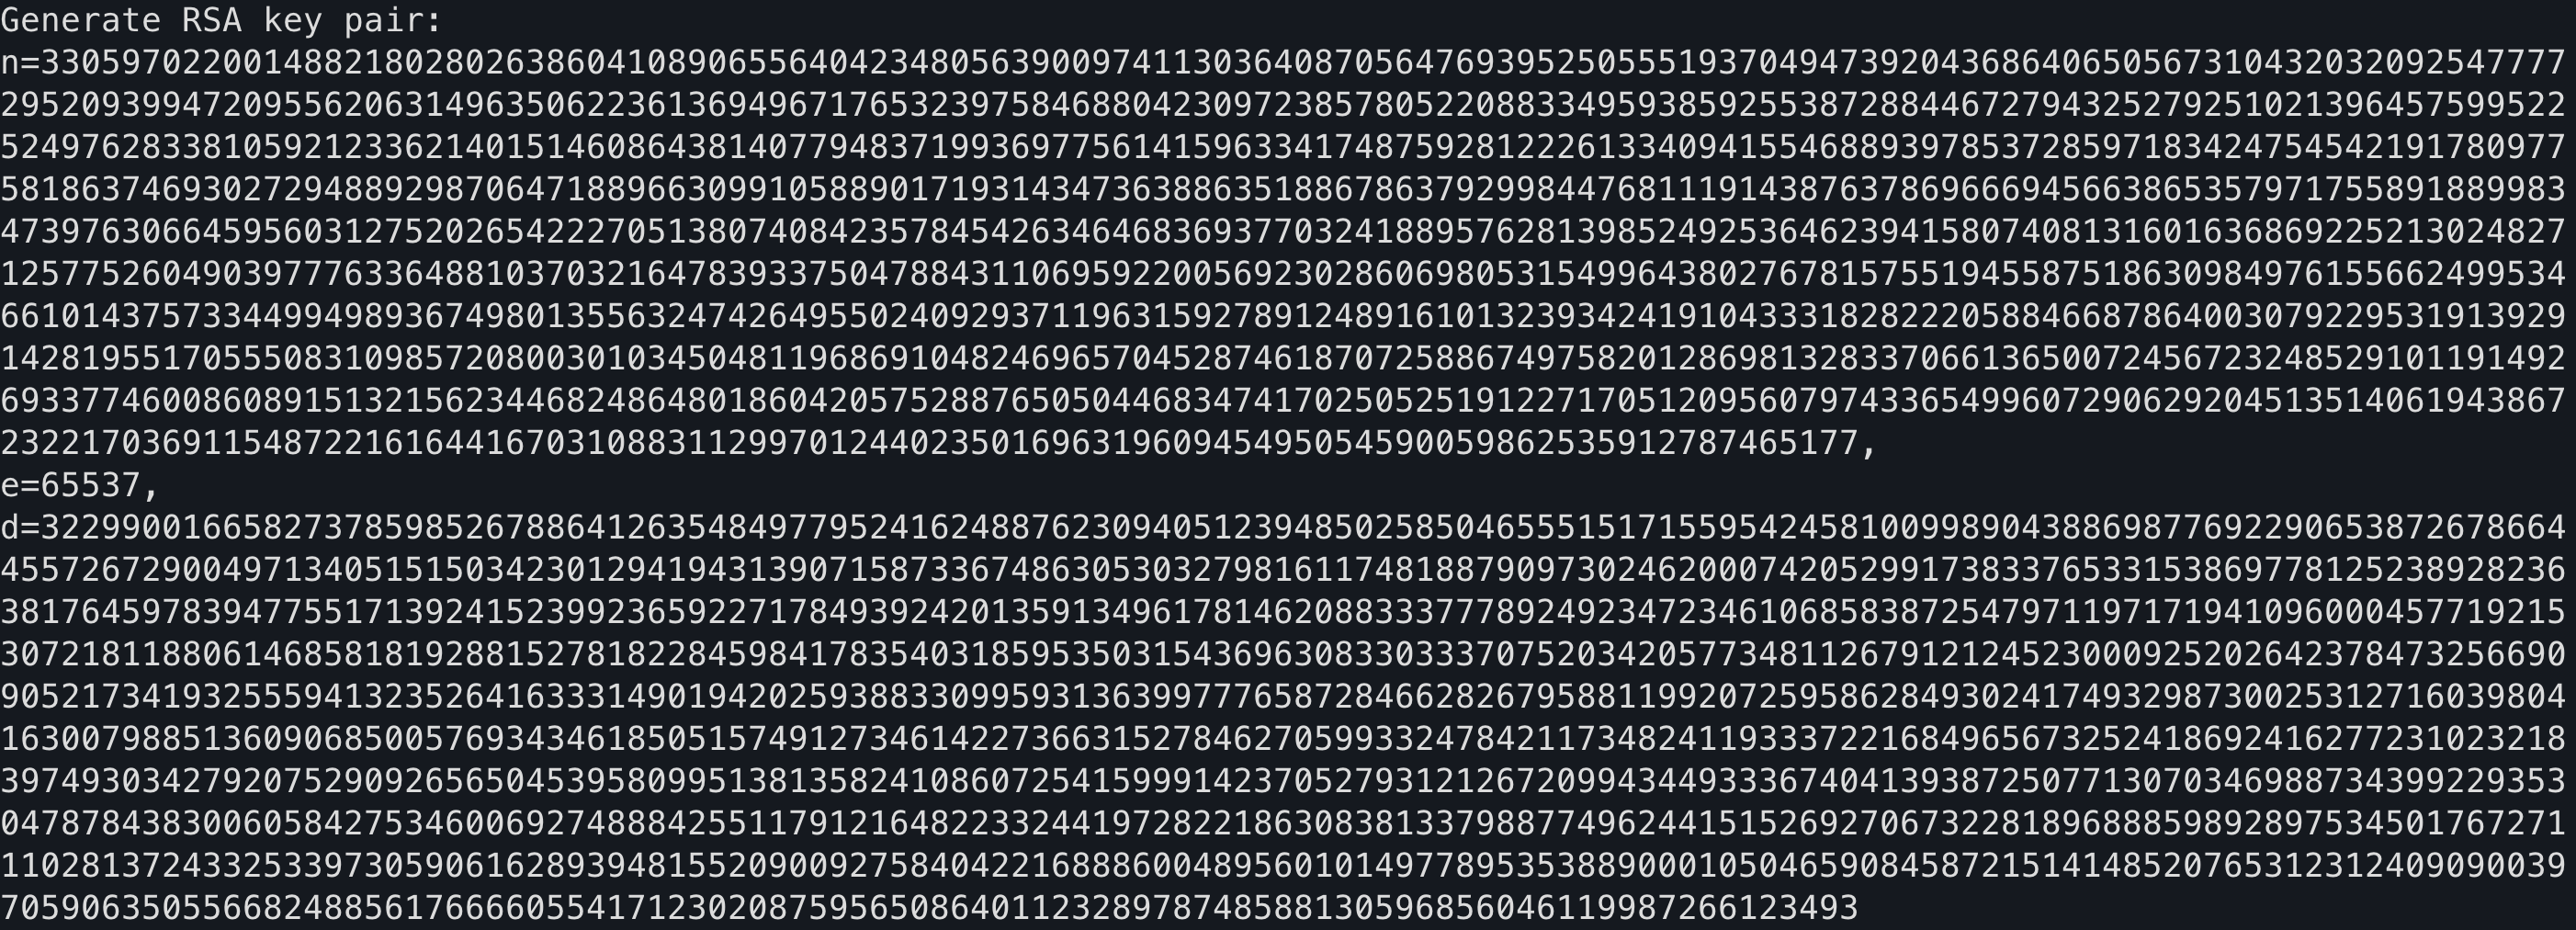
\includegraphics[width=\linewidth]{rsa_t1.png}
  \caption{密钥生成运行结果}
  \label{fig:t1}
\end{figure}

RSA 的实现跟之前 AES 的实现都使用 cargo 组织项目代码。
编译运行的代码:

  \begin{minted}[texcomments,tabsize=2,fontsize=\footnotesize,style=friendly,bgcolor=friendlybg]{bash}
  cd target/release && cargo build --release && ./crypto
  \end{minted}

密钥生成的 $n, e, d$ 如图~\ref{fig:t1} 所示,其中 $n$ 是两个 2048 位随机大素数 $p, q$ 的乘积, $e$ 则是固定的。

\section{公钥加密}

本题使用公钥对明文进行加密,明文为 'Cryptography and Network Security;学号;姓名拼音' ,使用自己的学号和姓名拼音替代对应位置字符串。加密过程包括分块,字符串转数字,公钥加密。分块将待加密的字符串分解成多个块,对于每个块分别加密。每个块的长度取决于选择的大素数p和q的大小,具体来说,比特串的长度应当小于log2n。块长度不足的部分需要使用填充字符补齐。字符串转数字可以先转化成比特串,再转化为数字,或者采用自行规定的转化规则。公钥加密部分请使用快速幂算法计算密文。输出每一步的结果。

\subsection{快速幂算法}
快速幂算法就是对计算 $m^e$ 的优化,就是把 $e$ 以二进制表示,复杂度 $O(2\log(n))$.
实现代码如下:

  \begin{minted}[texcomments,tabsize=2,fontsize=\footnotesize,style=friendly,bgcolor=friendlybg]{rust}
fn quick_pow_mod(mut m: Integer, e: &Integer, n: &Integer) -> Integer {
  m %= n;
  let mut ans = Integer::from(1);
  let mut e_curr = Integer::from(e);
  let two = Integer::from(2);
  while e_curr.significant_bits() != 0 {
      if e_curr.get_bit(0) {
          ans *= &m; ans %= n;
      }
      m.pow_mod_mut(&two, n).unwrap();
      e_curr >>= 1;
  }
  ans
}
  \end{minted}

\subsection{加密填充字符}

首先计算 $\log_2 n$ 作为加密块的大小,因为 $n$ 为 4096 位,也就是每一块为 512 字节。
对于明文的最后一块不足 512 字节的话,在最后面填充 0.
对于每一块的加密,就是把这一块当做一个大整数 $m$, 然后计算 $m^e \text{ mod } n$.
其中 $e, n$ 为公钥对。
代码如下:

  \begin{minted}[texcomments,tabsize=2,fontsize=\footnotesize,style=friendly,bgcolor=friendlybg]{rust}
fn rsa_encrypt(key: (&Integer, &Integer), plaintext: &str) -> Vec<u8> {
    let (n, e)  = key;
    let block_size = (n.significant_bits() as f64 / 8.0).ceil() as usize;
    let mut padded_bytes: Vec<u8> = plaintext.to_string().into_bytes();
    let mut pad_size = padded_bytes.len() % block_size;
    if pad_size != 0 {
        pad_size = block_size - pad_size;
    }
    println!("padding_size={}", pad_size);
    padded_bytes.extend(vec![PAD_BYTE; pad_size]);
    for block in padded_bytes.chunks_mut(block_size) {
        let mut num_str = block.iter()
            .map(|x| format!("{:02X}", x))
            .fold(String::from(""),
                  |res: String, curr: String| res + &curr
            );
        let mut m = Integer::from(Integer::parse_radix(
            num_str, 16).unwrap());
        m = quick_pow_mod(m, e, n);
        let mut digits = m.to_string_radix(16);
        if digits.len() % 2 == 1 { digits.insert(0, '0'); }
        for idx in 0..block.len() {
            block[idx] = u8::from_str_radix(&digits[
              (idx*2)..(idx*2+2)], 16).unwrap();
        }
    }
    padded_bytes
}
\end{minted}

\subsection{运行结果}

\begin{figure}[h]
\centering%
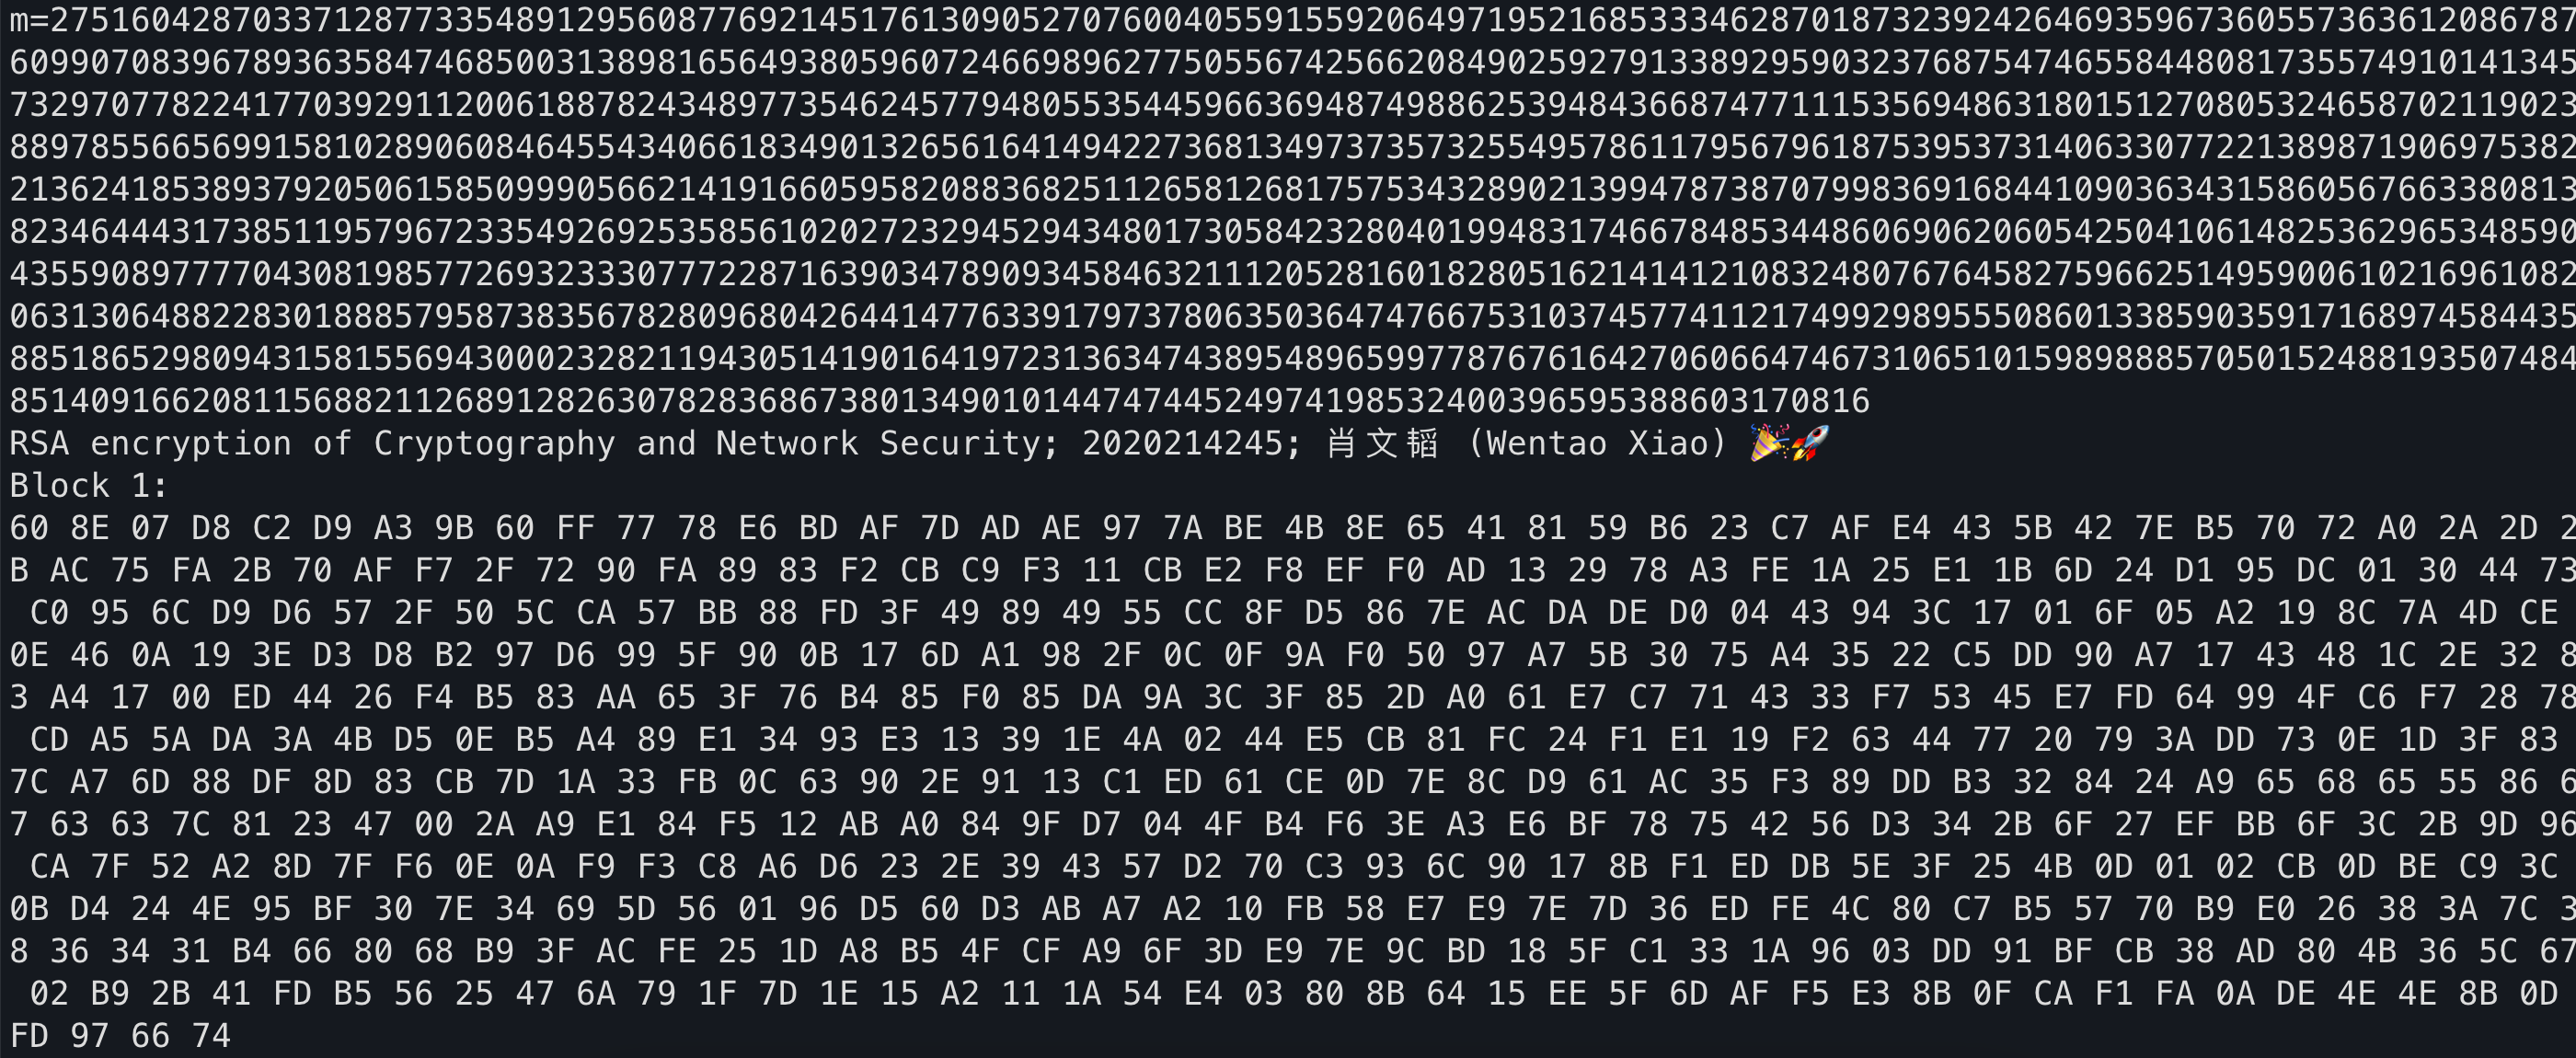
\includegraphics[width=\linewidth]{rsa_t2.png}
  \caption{公钥加密运行结果}
  \label{fig:t2}
\end{figure}

运行结果如图~\ref{fig:t2}所示,明文为“Cryptography and Network Security; 2020214245; 肖文韬 (Wentao Xiao) 🎉🚀”,加密结果为一个加密块。
值得一提的是,虽然明文对应的块大部分内容都是填充字符,但是加密块就是全满(没有填充字符)的数据。

\section{私钥解密}

私钥解密是公钥加密操作的逆操作,首先需要将比特串转化为数字,然后对数字使用私钥d进行解密,同样建议使用快速幂等算法计算,然后将数字还原成字符串,输出每一步的结果。

\subsection{代码说明}

因为 RSA 加密解密差不多一模一样,而且都能简单。
解密过程就是就是计算 $c^d \text{ mod } n$,其中 $c, d, n$ 分别为密文(块),私钥对。
去除填充字符的过程也比较简单,因为填充的字符就是 0,所以只需要把最后一块最后面连续的 0 去掉就好啦。

完整的代码如下:

  \begin{minted}[texcomments,tabsize=2,fontsize=\footnotesize,style=friendly,bgcolor=friendlybg]{rust}
fn rsa_decrypt(key: (&Integer, &Integer), cipher: &Vec<u8>) -> String {
    title("decryption");
    let (n, d) = key;
    let block_size = (n.significant_bits() as f64 / 8.0).ceil() as usize;
    let chunks = cipher.chunks(block_size);
    let num_chunks = chunks.len();
    let mut plain = String::new();
    for (idx, block) in chunks.enumerate() {
        let mut num_str = block.iter()
            .map(|x| format!("{:02X}", x))
            .fold(String::from(""),
                  |res: String, curr: String| res + &curr);
        if num_str.as_bytes()[0] == '0' as u8 {
            num_str.remove(0); }
        let mut c = Integer::from(Integer::parse_radix(
            num_str, 16).unwrap());
        println!("c={}", c);
        c = quick_pow_mod(c, d, n);
        let mut digits = c.to_string_radix(16);
        if digits.len() % 2 == 1 {
            digits.insert(0, '0'); }
        let mut c_block = vec![0u8; digits.len() / 2];
        for idx in 0..(digits.len() / 2) {
            c_block[idx] = u8::from_str_radix(&digits[(idx*2)..(idx*2+2)],
              16).unwrap(); }
        if idx == (num_chunks - 1) {
            while c_block[c_block.len() - 1] == PAD_BYTE {
                c_block.pop(); } }
        plain.push_str(&String::from_utf8(c_block).unwrap());
    }
    plain
}
\end{minted}

\subsection{运行结果}

\begin{figure}[h]
\centering%
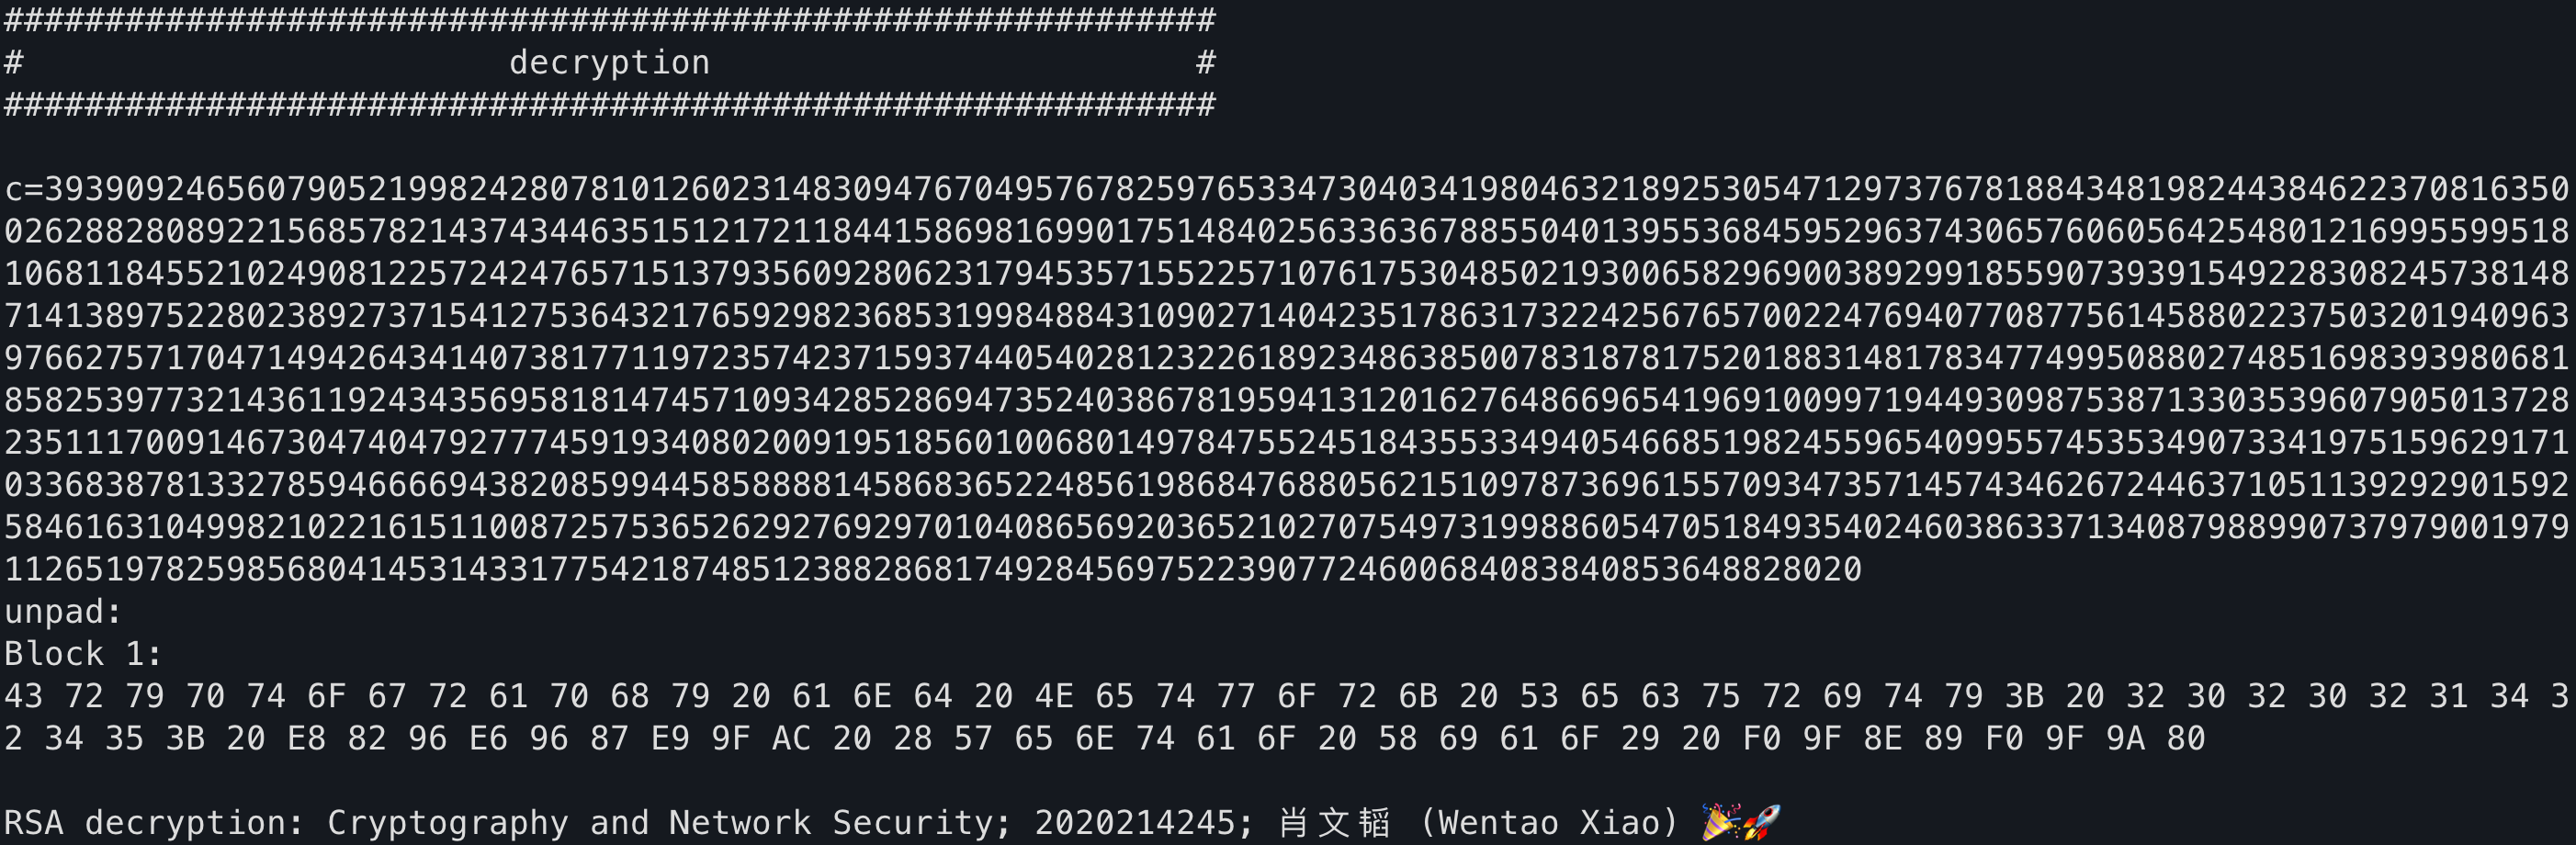
\includegraphics[width=\linewidth]{rsa_t3.png}
  \caption{私钥解密运行结果}
  \label{fig:t3}
\end{figure}

运行结果如图~\ref{fig:t3}所示,解密出来的明文为“Cryptography and Network Security; 2020214245; 肖文韬 (Wentao Xiao)”。
解密出来的块当中大部分为填充字符。

\section{数字签名}

签名的内容可以和题目2中使用的字符串相同,也可以是从文件中导入的任意一个字符串。

签名过程主要包括消息散列,私钥加密,验证过程包括公钥解密,对比验证。首先需要将字符串压缩成哈希值,在这一环节中允许使用现有的哈希函数库,Python中的哈希函数库为hashlib。私钥加密和公钥解密的过程同题目2和3,使用题目1中生成的密钥对,注意要使用私钥加密,公钥解密,与题目2和3中是相反的,输出每一步的结果。

\subsection{代码说明}

值得注意的是,RSA在传输加密的数据的时候,发送者要用接受者的公钥加密消息,然后用发送者自己的私钥签名(加密)明文消息与密文一起发送给接受者。
因为数字签名就是加密,只不过用的秘钥不一样,所以代码实现还是很简单的。
代码如下:

  \begin{minted}[texcomments,tabsize=2,fontsize=\footnotesize,style=friendly,bgcolor=friendlybg]{rust}
fn rsa_sign(plaintext: &str) -> (Integer, Integer, Vec<u8>, String) {
    let (n, e, d) = rsa_key_pair("extend_gcd")
    let cipher = rsa_encrypt((&n, &d), plaintext);
    let mut hasher = DefaultHasher::new();
    plaintext.hash(&mut hasher);
    let hash: u64 = hasher.finish();
    let sign = quick_pow_mod(Integer::from(hash), &d, &n)
      .to_string_radix(16);
    (n, e, cipher, sign)
}

fn rsa_check_sign(cipher: &Vec<u8>, n: &Integer, e: &Integer,
                  sign: &str, plain: &str) -> bool {
    let decrypted = rsa_decrypt((n, e), cipher);
    let mut hasher = DefaultHasher::new();
    decrypted.hash(&mut hasher);
    let hash: u64 = hasher.finish();
    let hash_in_sign: u64 = quick_pow_mod(
        Integer::from(Integer::parse_radix(sign, 16).unwrap()),
        e, n).to_u64().unwrap();
    hash == hash_in_sign
}
\end{minted}

\subsection{运行结果}

\begin{figure}[h]
\centering%
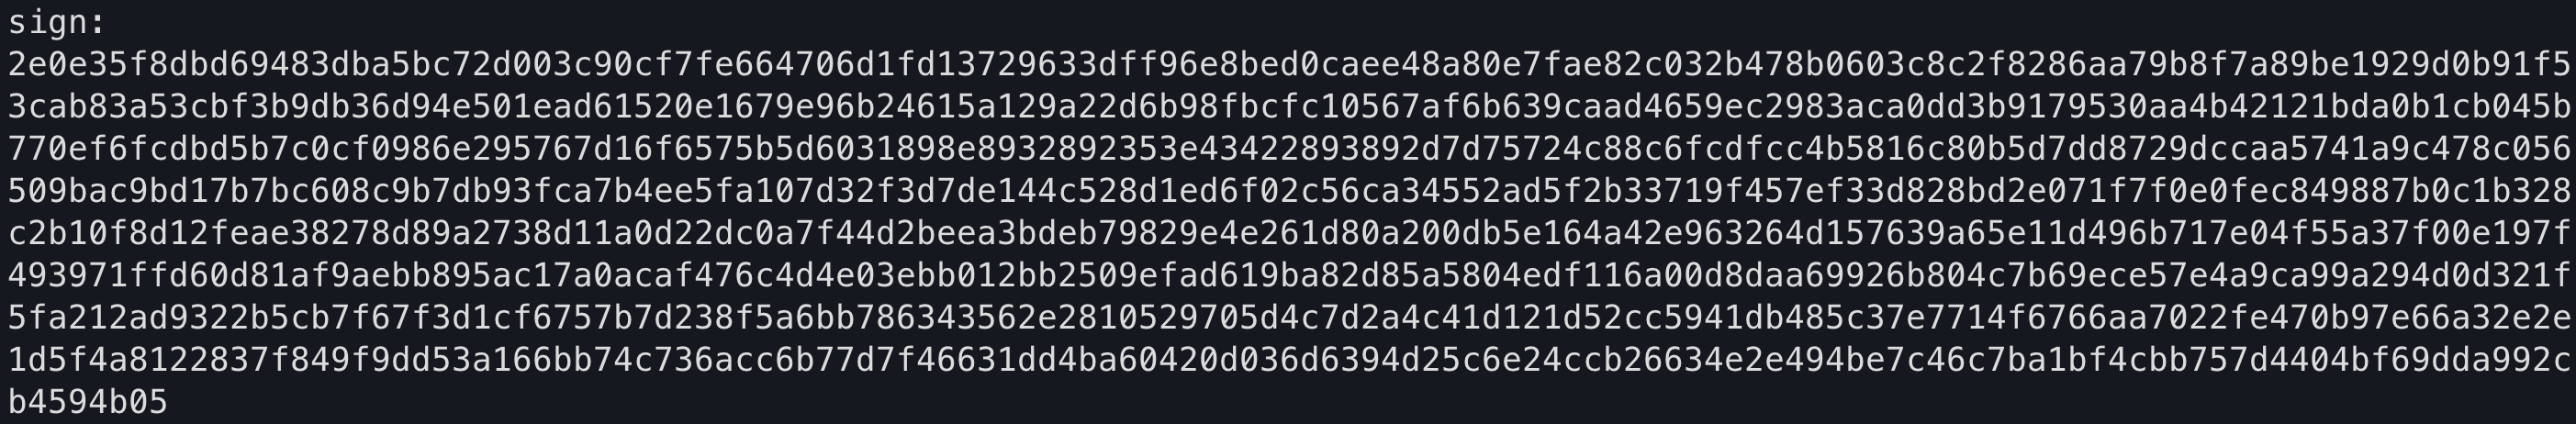
\includegraphics[width=\linewidth]{rsa_t4.png}
  \caption{数字签名运行结果}
  \label{fig:t4}
\end{figure}

对消息“Cryptography and Network Security; 2020214245; 肖文韬 (Wentao Xiao)”的RSA数字签名,运行结果如图~\ref{fig:t4}所示。


% 其他部分
\backmatter

% 参考文献
% \bibliography{ref/refs}  % 参考文献使用 BibTeX 编译

\end{document}
